\documentclass[journal]{IEEEtran}

\usepackage{preamble}
\usepackage{abbreviation} % Liste des abréviations
\usepackage{authblk}

\title{New wideband large aperture open-ended coaxial microwave probe for soil dielectric characterization}

% \title{Calibration of a wide-band large open-ended coaxial probe and usage example for soil sample dielectric caracterization}

% Remove date from title
\date{}

\author[1,2]{Alex Gélinas}
\author[3]{Bilal Filali}
\author[2,4]{Alexandre Langlois}
\author[5]{Richard Kelly}
\author[1,2]{Alex Mavrovic}
\author[6]{François Demontoux}
\author[1,2]{Alexandre Roy}

\affil[1]{Centre de recherche sur les interactions bassins versants – écosystèmes aquatiques (RIVE), Université du Québec à Trois-Rivières}
\affil[2]{Centre d'Études Nordiques (CEN), Université Laval}
\affil[3]{PhyVertX Technologies Inc.}
\affil[4]{Centre d'Applications et de Recherches en Télédétetcion (CARTEL), Université de Sherbrooke}
\affil[5]{Department of Geography and Environmental Management, University of Waterloo}
\affil[6]{Laboratoire de l'Intégration du Matériau au Système (IMS), Université de Bordeaux}
\setcounter{Maxaffil}{0}
\renewcommand\Affilfont{\itshape\small}% checktex 6



\usepackage[style=ieee,
            backref=false,
            isbn=false,
            eprint=false,
            url=false,
            doi=false,
            ]{biblatex}
\addbibresource{bib/_ProbePermittivity.bib}

\AtEveryBibitem{\clearfield{month}}
\AtEveryCitekey{\clearfield{month}}

% Diagonal fraction
\newcommand{\sidefrac}[2]{{}^{#1}{\mskip-3mu/\mskip-3mu}_{#2}}

% From IEEE how-to.tex
\usepackage{balance}

\begin{document}

\maketitle

\begin{abstract}
    We present a unique Open-Ended Coaxial Probe that has the capability of accurately measuring the permittivity of heterogeneous materials, such as soil, due to its large aperture.
    The probe was designed to work at frequencies ranging from \qtyrange{0.5}{18}{\giga\hertz}, which is a particularly important range for microwave remote sensing applications, and more precisely the \ac{tsmm}.
    \ac{tsmm} aims at launching a new satellite equipped with a dual Ku-band radar (\qtyrange[range-phrase=~and~]{13.5}{17.2}{\giga\hertz}) for snow monitoring.
    At Ku-band frequencies, the backscattered radar signal contains information about the snow, but can also contain a contribution from the soil.
    Knowing the soil permittivity will enable a better representation of this soil contribution to the radar signal to obtain more accurate snow data such as \ac{swe}.
    To demonstrate the accuracy and repeatability of the probe, solutions of known permittivity were measured, and the results were compared to their theoretical values.
    Then, tests for approximating the penetration depth of the probe signal were conducted with dry and wet paper.
    Afterwards, a protocol to use the probe to compute the permittivity of soil samples in freeze/thaw cycles was developed.
    The permittivity of commercial sand and arctic organic soil from Cambridge Bay (Nunavut) are presented for different relevant microwave remote sensing frequencies selected on the full range of the probe and temperatures (\qtyrange{-20}{20}{\degreeCelsius}) according to the new protocol.
    The main goal of this paper is to present the probe and its potential use in the field of remote sensing, especially for active Ku-band remote sensing applications, where there is little work done.
\end{abstract}

\begin{IEEEkeywords}
    Coaxial probe, Microwaves, Remote Sensing, Permittivity, Soil
\end{IEEEkeywords}

\section{Introduction}

\IEEEPARstart{R}{ecent developments} in active microwave remote sensing showed the potential of \ac{sar} for monitoring important snow characteristics.
More precisely, studies demonstrated the high sensitivity of \ac{sar} backscattering in the Ku-band domain (\qtyrange{12}{18}{\giga\hertz}) to \acf{swe} \parencite{Shi2016,King2018,Rutter2019}.
Following \ac{swe} temporal and spatial variation in location where the snow coverage spans more than 6 months per year is of utmost importance for hydrological cycles \parencite{Zhang2005,Ayguen2020}, surface energy balance \parencite{Cohen2001,Box2019} and biogeochemical cycles \parencite{Zhang2005,Grogan2006}, among others.
The significance of seasonal snowmelt and \ac{swe} in delivering freshwater is of great importance for the well-being of Canadians, supporting a diverse array of economic sectors and sustaining ecosystems.
Simultaneously, it introduces risks through contributions to floods and the perpetuation of drought events.
The impact of these snow variables, combined with the recent \ac{sar} developments led to the beginning of a joint mission from \ac{csa} and \ac{eccc}, \acf{tsmm} \parencite{Derksen2019,Garnaud2019}, which aims to launch a dual Ku-band \ac{sar} (\qty{13.5}{\giga\hertz} and \qty{17.2}{\giga\hertz}) aboard a satellite for snow monitoring in the Northern Hemisphere.
Moreover, satellite Ku-band \ac{sar} observations would offer regular high resolution (few meters) \ac{swe} data for remote locations around the globe, under various meteorological conditions \parencite{Tsai2019}.
Indeed, Ku-band radar signals have low interactions with atmospheric particles such as water vapor in clouds and is completely independent of solar radiations.

However, there are still lots of challenges for \ac{swe} inversion using the Ku-band \ac{sar} backscatter signal.
Indeed, the backscattering signal is not only influenced by \ac{swe}, but also by other snowpack characteristics such as microstructure and liquid water content, and by the substrate under the snow (sea ice, fresh water ice, soil, etc.) and vegetation cover.
To overcome these obstacles, modelization of the signal via microwave radiative transfer models such as \ac{smrt} \parencite{Picard2018} is used to disentangle the effect from each contribution, enabling \ac{swe} retrieval from the backscattering signal.
Most of the existing models for active remote sensing backscatter were built for lower microwave frequencies (\(<\)\qty{6}{\giga\hertz}, \parencite{Longepe2009}), whereas \ac{smrt} was designed to work in a frequency range that encompasses the \ac{tsmm} mission dual Ku-band frequencies.
Moreover, \ac{smrt} was specifically conceived to include parameters such as snow microstructure and the substrate characteristics.
Nonetheless, \ac{smrt} developers note that there is a need for more precise wave diffusion models at snow/substrate interface \parencite{Picard2018}.
Soil contribution remains misrepresented by the model and brings some uncertainty in the snow signal produced \parencite{King2018}.
In order to model the soil contribution to the total backscattering signal, an important parameter to understand is the soil relative permittivity (hereafter referred to as permittivity).

Knowing the soil permittivity allows to model the soil influence over the total signal.
In current radiative transfer models targeting snow characteristics, frozen soil permittivity is often set to a constant close to that of dry soil \parencite{Hallikainen1985,Kerr2012}.
This is due to the lack of knowledge regarding the spatial and temporal variability of frozen soil permittivity.
Soil permittivity greatly depends on soil water content \parencite{Topp1980} where water permittivity is relatively high (\(\varepsilon^\prime \approx 80\) at L-band) compared to dry soil (\(\varepsilon^\prime \approx 2.5\) \parencite{Matzler1998}) or ice (\(\varepsilon^\prime \approx 3.2\) \parencite{Matzler1987}).
This means that having unfrozen water in the soil would greatly increase the permittivity, hence modifying the soil backscattering signal.
Previous work on soil dielectric properties have been made where the dielectric constant is measured as a function of either the temperature and/or the water content and the soil texture \parencite{Cihlar1974,Hoekstra1974,Bobrov2015,Kabir2020}.
Models for soil permittivity (called dielectric mixing models, \parencite{Dobson1985,Hallikainen1985,Mironov2009,Zhang2010}) have also previously been developed.%

In this context, the goal of this article is to present a novel \ac{oecp} with an operating frequency range from \SIrange{0.5}{18}{\giga\hertz}, able to measure the permittivity of a flat material or liquid.
The probe aperture (the measurement plane) is sufficiently large to integrate a representative average permittivity over non-homogeneous soil.
The experimental setup required to operate the probe is simple and easily portable, making it perfect for laboratory or field usage.
In this study, we present the novel \ac{oecp} and its precision over its full operating range as well as tests to estimate the probe signal penetration depth.
Then, liquids of known permittivity are used to compare the probe's results to theoretical values in order to validate the probe calibration.
Finally, a protocol was developed to measure the soil permittivity in a controlled varying temperature environment (from \qtyrange{-20}{20}{\degreeCelsius}).
Two different soil types (sand and arctic organic soil) were analyzed following the new protocol.

\section{Theory and methodology}\label{sec:metho}

\subsection{Probe setup}\label{subsec:metho-mats}
The \ac{oecp} used in this project was developed by PhyVertX Technologies Inc., and is an adaptation for higher frequencies of the probe described in \parencite{Filali2008}. 
The probe was tested on different substrates such as vegetation, snow and ice, and soil \parencite{Mavrovic2018,Mavrovic2020,Mavrovic2021}.
The probe is made of two conducting coaxial cylinders with a \ac{ptfe} core akin to a coaxial cable.
The inner cylinder has a \(2a =\) \SI{4}{\mm} diameter while the outer cylinder has a \(2b =\) \SI{13.2}{\mm} diameter (Figure~\ref{fig:probe-scheme}A).

\begin{figure}[ht!]
    \centering
    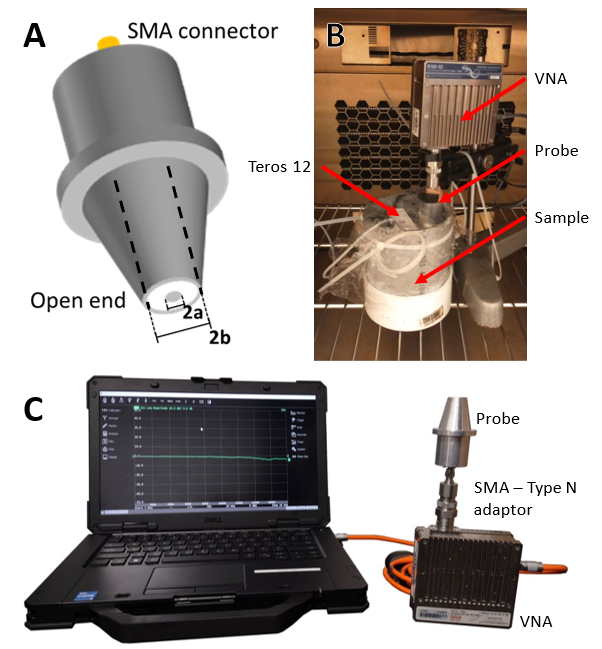
\includegraphics[width=0.9\columnwidth]{Images/method-pic.png}
    \caption[]{\textbf{A:} \ac{oecp} schematic, where the diameter of the conductive core (2a) is \qty{4}{\milli\meter} and the outer diameter of the PTFE core (2b) is \qty{13.2}{\milli\meter}; \textbf{B:} Experimental setup for the temperature cycle measures; \textbf{C:} \ac{vna} and \ac{oecp}, connected to the computer with the operating software for the \ac{vna}}\label{fig:probe-scheme}
\end{figure}

The probe aperture is large enough to measure heterogeneous material, such as soil, while being able to cover a frequency range from \SI{0.5}{\giga\hertz} up to \SI{18}{\giga\hertz}.
To operate the \ac{oecp}, we used a 1-port \ac{vna}\textemdash the R180 (\SIrange{0.001}{18}{\giga\hertz}, frequency resolution of \qty{50}{\hertz})\textemdash from Copper Mountain\(^\text{\textregistered}\) Technologies.
All the instruments, connectors and cables in the setup have an impedance of \SI{50}{\ohm} to reduce unwanted reflections.
To connect the \ac{oecp} (SMA connector) to the \ac{vna} (Type-N connector), using a solid adaptor allows eliminating the noise that could occur in cables or semi-rigid adaptors.
The \ac{vna} was then connected to a computer and was operated by the company's RVNA software (Figure~\ref{fig:probe-scheme}C).
Once the setup completed, two calibrations were performed to ensure measurements accuracy: the first calibrates the cables and connectors plugged on the probe using a specific calibration kit (system calibration) and the second calibrates the probe measurement plane, i.e., probe aperture (probe calibration, see Section~\ref{subsec:metho-calib} for more details).

\subsection{Probe measurement principle}\label{metho:probe-princip}
To obtain the permittivity at the probe's aperture, the \ac{vna} measures the reflection coefficient \(\rho\).
The measure is then linked to the real reflection coefficient \(\Gamma\) through the probe's scattering parameters with the Equation~\ref{eq:gamma-sij} \parencite{Nyshadham1992}:
%
\begin{equation}\label{eq:gamma-sij}
    \Gamma = \frac{\rho-S_{11}}{S_{22}\rho+S_{12}S_{21}-S_{11}S_{22}}
\end{equation}
%
where the \(S_{i,j} \left(i,j \in \left\{1,2\right\}\right)\) are the probe scattering parameters.
The probe calibration, detailed in Section~\ref{subsec:metho-calib}, is made to find those \(S_{i,j}\) using liquids of known permittivity.
\(\Gamma\) is also related to the admittance of both the probe (\(Y_0\)) and the material under test (\(Y(\varepsilon)\)) with Equation~\ref{eq:gamma-admit} \parencite{Nyshadham1992}:
%
\begin{equation}\label{eq:gamma-admit}
    \Gamma = \frac{Y(\varepsilon) - Y_0}{Y(\varepsilon) + Y_0}
\end{equation}
%
Finally, the medium's permittivity (\(\varepsilon_r\)) can be deduced from its admittance (\(Y(K)\)) with Equation~\ref{eq:probe-permittivity} \parencite{Galejs1969a}:
%
\begin{equation}\label{eq:probe-permittivity}
    Y(K) = \frac{\varepsilon_r Z_\nu}{\ln(\sidefrac{a}{b})} 
    \int_{0}^{\infty}
    \frac{{\left[J_0(\beta p)-J_0(\alpha p)\right]}^2} % checktex 3
         {p\sqrt{\varepsilon_r - p^2}}dp
\end{equation}
%
where \(K=\sidefrac{2\pi f}{c}\) is the wave number in vacuum, \(Z_\nu=\sqrt{\sidefrac{\mu_{0}}{\varepsilon_{0}}}\approx \qty{376.7303}{\ohm}\) is the vacuum impedance, \(\alpha = Ka\), \(\beta = Kb\) are geometric parameters, \(J_{0}\) is the zero\textsuperscript{th} order Bessel function of the first kind and \(p\) is the integration variable.  % related to the sine and cosine directors: \(p^2=u^2+v^2\).

\subsection{Calibration}\label{subsec:metho-calib}
The calibration principle is based on the \ac{sol} one-port method, where measurements of known standards are compared to their theoretical values for all three calibration standards (open, short-circuit and load).
The measurements are then processed to find the \(S_{i,j}\) (Equation~\ref{eq:gamma-sij}) parameters of the calibration plane.
%To obtain accurate measurements, two calibrations are necessary: first, a system calibration at the probe connection plane to calibrate the \ac{vna} and the connectors and cables connected to the probe.
To obtain accurate measurements, two calibrations are necessary: first, a system calibration at the probe connection plane and second, a probe calibration at the measurement plane.
This first system calibration is performed using a S2611 calibration kit from Copper Mountain\(^\text{\textregistered}\) Technologies and ensures that the \ac{vna} and the connectors and cables are calibrated.
The kit includes all the necessary standards and has a \SI{50}{\ohm} impedance.
Once the system is calibrated, the probe is connected at the end of the line and the second calibration is done.
The probe calibration was designed specifically for the probe using the \ac{sol} method at the measurement plane (the aperture).
The open standard corresponds to a measure in the air, the short-circuit standard was made by covering the probe with a conducting metal such as copper and the load standard was a saline (NaCl) water solution (\qty{35}{ppt}).

Using these three standards, Equation~\ref{eq:gamma-sij} can be written for each \(\rho_{1,2,3}\) and \(\Gamma_{1,2,3}\), where \(\Gamma_{1,2,3}\) is deduced from \(Y_{1,2,3}\) using Equation~\ref{eq:gamma-admit}.
Solving these three equations leads to a system of three equations for three unknown variables (Equation~\ref{eq:sij-system}):

{\footnotesize
\begin{equation*}
    S_{11} = \frac{\Gamma_1\Gamma_2\rho_3(\rho_1-\rho_2) + 
                   \Gamma_1\Gamma_3\rho_2(\rho_3-\rho_1) + 
                   \Gamma_2\Gamma_3\rho_1(\rho_2-\rho_3)}
                  {\Gamma_1\Gamma_2(\rho_1-\rho_2) + 
                   \Gamma_1\Gamma_3(\rho_3-\rho_1) +
                   \Gamma_2\Gamma_3(\rho_2-\rho_3)}
\end{equation*}
%
\begin{equation}\label{eq:sij-system}
    S_{22} = \frac{\Gamma_1(\rho_2-S_{11}) + \Gamma_2(S_{11}-\rho_1)}       
                  {\Gamma_1\Gamma_2(\rho_2-\rho_1)}
\end{equation}
%
\begin{equation*}
    S_{12}S_{21} = \frac{(\rho_1-S_{11})(1-S_{22}\Gamma_1)}{\Gamma_1}
\end{equation*}}%

After the probe calibration, two test liquids were used to assess the probe calibration quality.
The first test liquid was a saline solution at \qty{20}{ppm} and the second one was methyl hydrate.
Both computed permittivity were compared to the theoretical permittivity provided by \textcite{Nyshadham1992}.

\subsection{Data processing}\label{subsec:metho-smooth}
For every measurement presented in this work, the raw data frequency ranged from \SIrange{0.5}{18}{\giga\hertz} with increments of \SI{4}{\mega\hertz}. 
For the probe calibration and test liquids, the permittivity was computed using the full raw data range.
Afterwards, to accelerate the permittivity computation for the studied samples (wet and dry paper, wet and dry sand, and soil), the raw data was truncated so that the frequency increments were of \SI{100}{\mega\hertz} over the range of \SIrange{0.5}{18}{\giga\hertz}.
This reduced the dataset size, making the computation faster while keeping enough data points to represent the permittivity's possible variation.
With the permittivity computed, the results were smoothed using the rolling window average or the exponentially weighted moving average methods with a window size of \qty{8.33}{\percent} of the total range to improve the consistency between measurements.
% For the calibration liquids, the rolling window size was \SI{1492}{\mega\hertz} or \SI{373}{points} which corresponds to 1/12th or \SI{8.3333}{\percent} of the total frequency range (\SIrange{0.5}{18}{\giga\hertz} with steps of \SI{4}{\mega\hertz}).
% For the samples with \SI{100}{\mega\hertz} increments the same rolling window size of \SI{1492}{\mega\hertz} was used but consisted of \SI{15}{points} (1/12th of the total range).

% \subsection{Highlighted frequencies}\label{subsec:mehto-freq}
Since our probe covers a wide frequency range (from \qtyrange{0.5}{18}{\giga\hertz}), the analysis was made on specific frequencies used in \ac{swe} remote sensing.
In the context of the new satellite mission concept for \ac{swe} monitoring (\ac{tsmm}), the targeted frequencies were also added to the list (Table~\ref{tab:freq-range}).

\begin{table}[ht!]
    \centering
    \caption{Frequency bands (\qty{\pm0.25}{\giga\hertz}) on which the average permittivity was computed with examples of relevant satellite-based sensors}\label{tab:freq-range}
    \begin{tabular}{r l c c}
        Band & Frequency & Satellite example & Ref. \\
        \midrule\midrule
        L-band & \qty{1.5}{\giga\hertz} & SMOS (\qty{1.4}{\giga\hertz}) & \parencite{Kerr2010}\\
        C-band & \qty{6.9}{\giga\hertz} & RadarSAT (\qty{5.3}{\giga\hertz}) & \parencite{Morena2004} \\
        X-band & \qty{10.65}{\giga\hertz} & TerraSAR-X (\qty{9.65}{\giga\hertz}) & \parencite{Werninghaus2010} \\
        Ku-band 1 & \qty{13.5}{\giga\hertz} & TSMM (\qty{13.5}{\giga\hertz}) & \parencite{Derksen2019,Garnaud2019} \\
        Ku-band 2 & \qty{17.2}{\giga\hertz} & TSMM (\qty{17.2}{\giga\hertz}) & \\
    \end{tabular}
\end{table}

\subsection{Probe signal penetration depth}\label{subsec:metho-paper}
A test using stacked paper sheets allowed estimating the probe penetration depth \parencite{Elrayes1987}.
The process consisted in progressively stacking sheets of paper on top of a conductive metal plate (copper, high reflectivity).
Every few sheets of paper, a permittivity measurement of the paper stack (low relative permittivity) was made.
Once the measured permittivity remained constant for additional sheets of paper, the signal contribution from the conductive plate was assumed completely lost, yielding an estimation of the penetration depth of the probe signal.
This test was repeated for dry and wet paper on \qtyproduct{216 x 279}{\mm} (\qtyproduct{8.5 x 11}{in}) US letter size printer paper of \qty{0.1}{\milli\metre} thickness. % chktex 29

\subsection{Soil sample characterization}\label{subsec:metho-soil}
The probe was used to characterize dry and wet commercial sand and arctic organic mesic soil from Cambridge Bay (Nunavut, Canada, \ang{69.2275}, \ang{-104,8937}).
The arctic soil sample was collected using a cylindrical PVC soil sample holder of \qty{5}{\cm} radius and \qty{10}{\cm} height driven in the soil and excavated so the soil remained undisturbed.
The wet sand and organic soil samples were exposed to a temperature ramp from \qtyrange{-20}{20}{\degreeCelsius} over 10 hours inside a Climats EX-CAL 1411-HE climatic chamber at Laboratoire de l'Intégration du Matériau au Système (IMS, Bordeaux, France).
The wet sand and wet organic soil samples were placed in the convection centre of the climatic chamber (Figure~\ref{fig:probe-scheme}B).
A plastic wrap was used to seal the soil sample cylinder to ensure a constant soil moisture throughout all the temperature cycle.
To monitor the soil moisture and the soil temperature during the tests, a thermocouple connected to the test chamber was used, as well as a Teros 12 soil moisture and temperature probe (operating frequency of \qty{70}{\mega\hertz}, METER Group, Inc. USA).
The test chamber's thermocouple  length is approximately \qty{4}{\cm}.
The thermocouple was inserted in the top layer of the soil sample.

% The dry sand was also tested inside the climatic chamber using the temperature ramp and the same experimental setup, however, its permittivity did not fluctuate with temperate.
% Moreover, since the sand was tested in the climatic chamber, it was subjected to a constant flow of dried air.
% No plastic wrap was used to seal the sample holder to maintain the dryness.
% Hence, the dry sand permittivity results shown represent the real and imaginary permittivity over all the probe frequency range.

\section{Results and discussion}

\subsection{Probe calibration and test liquids}\label{subsec:res-calib}
The calibration curves with the test saline solution (\qty{20}{ppt}) and methyl hydrate largely agree with the theoretical values \parencite{Nyshadham1992} (Figure~\ref{fig:calib-results}), with a \ac{rmse} of \num{1.14} and \num{0.94} respectively.
Figure~\ref{fig:calib-results} also highlights the chosen frequency ranges for remote sensing applications.

\begin{figure}[ht!]
    \centering
    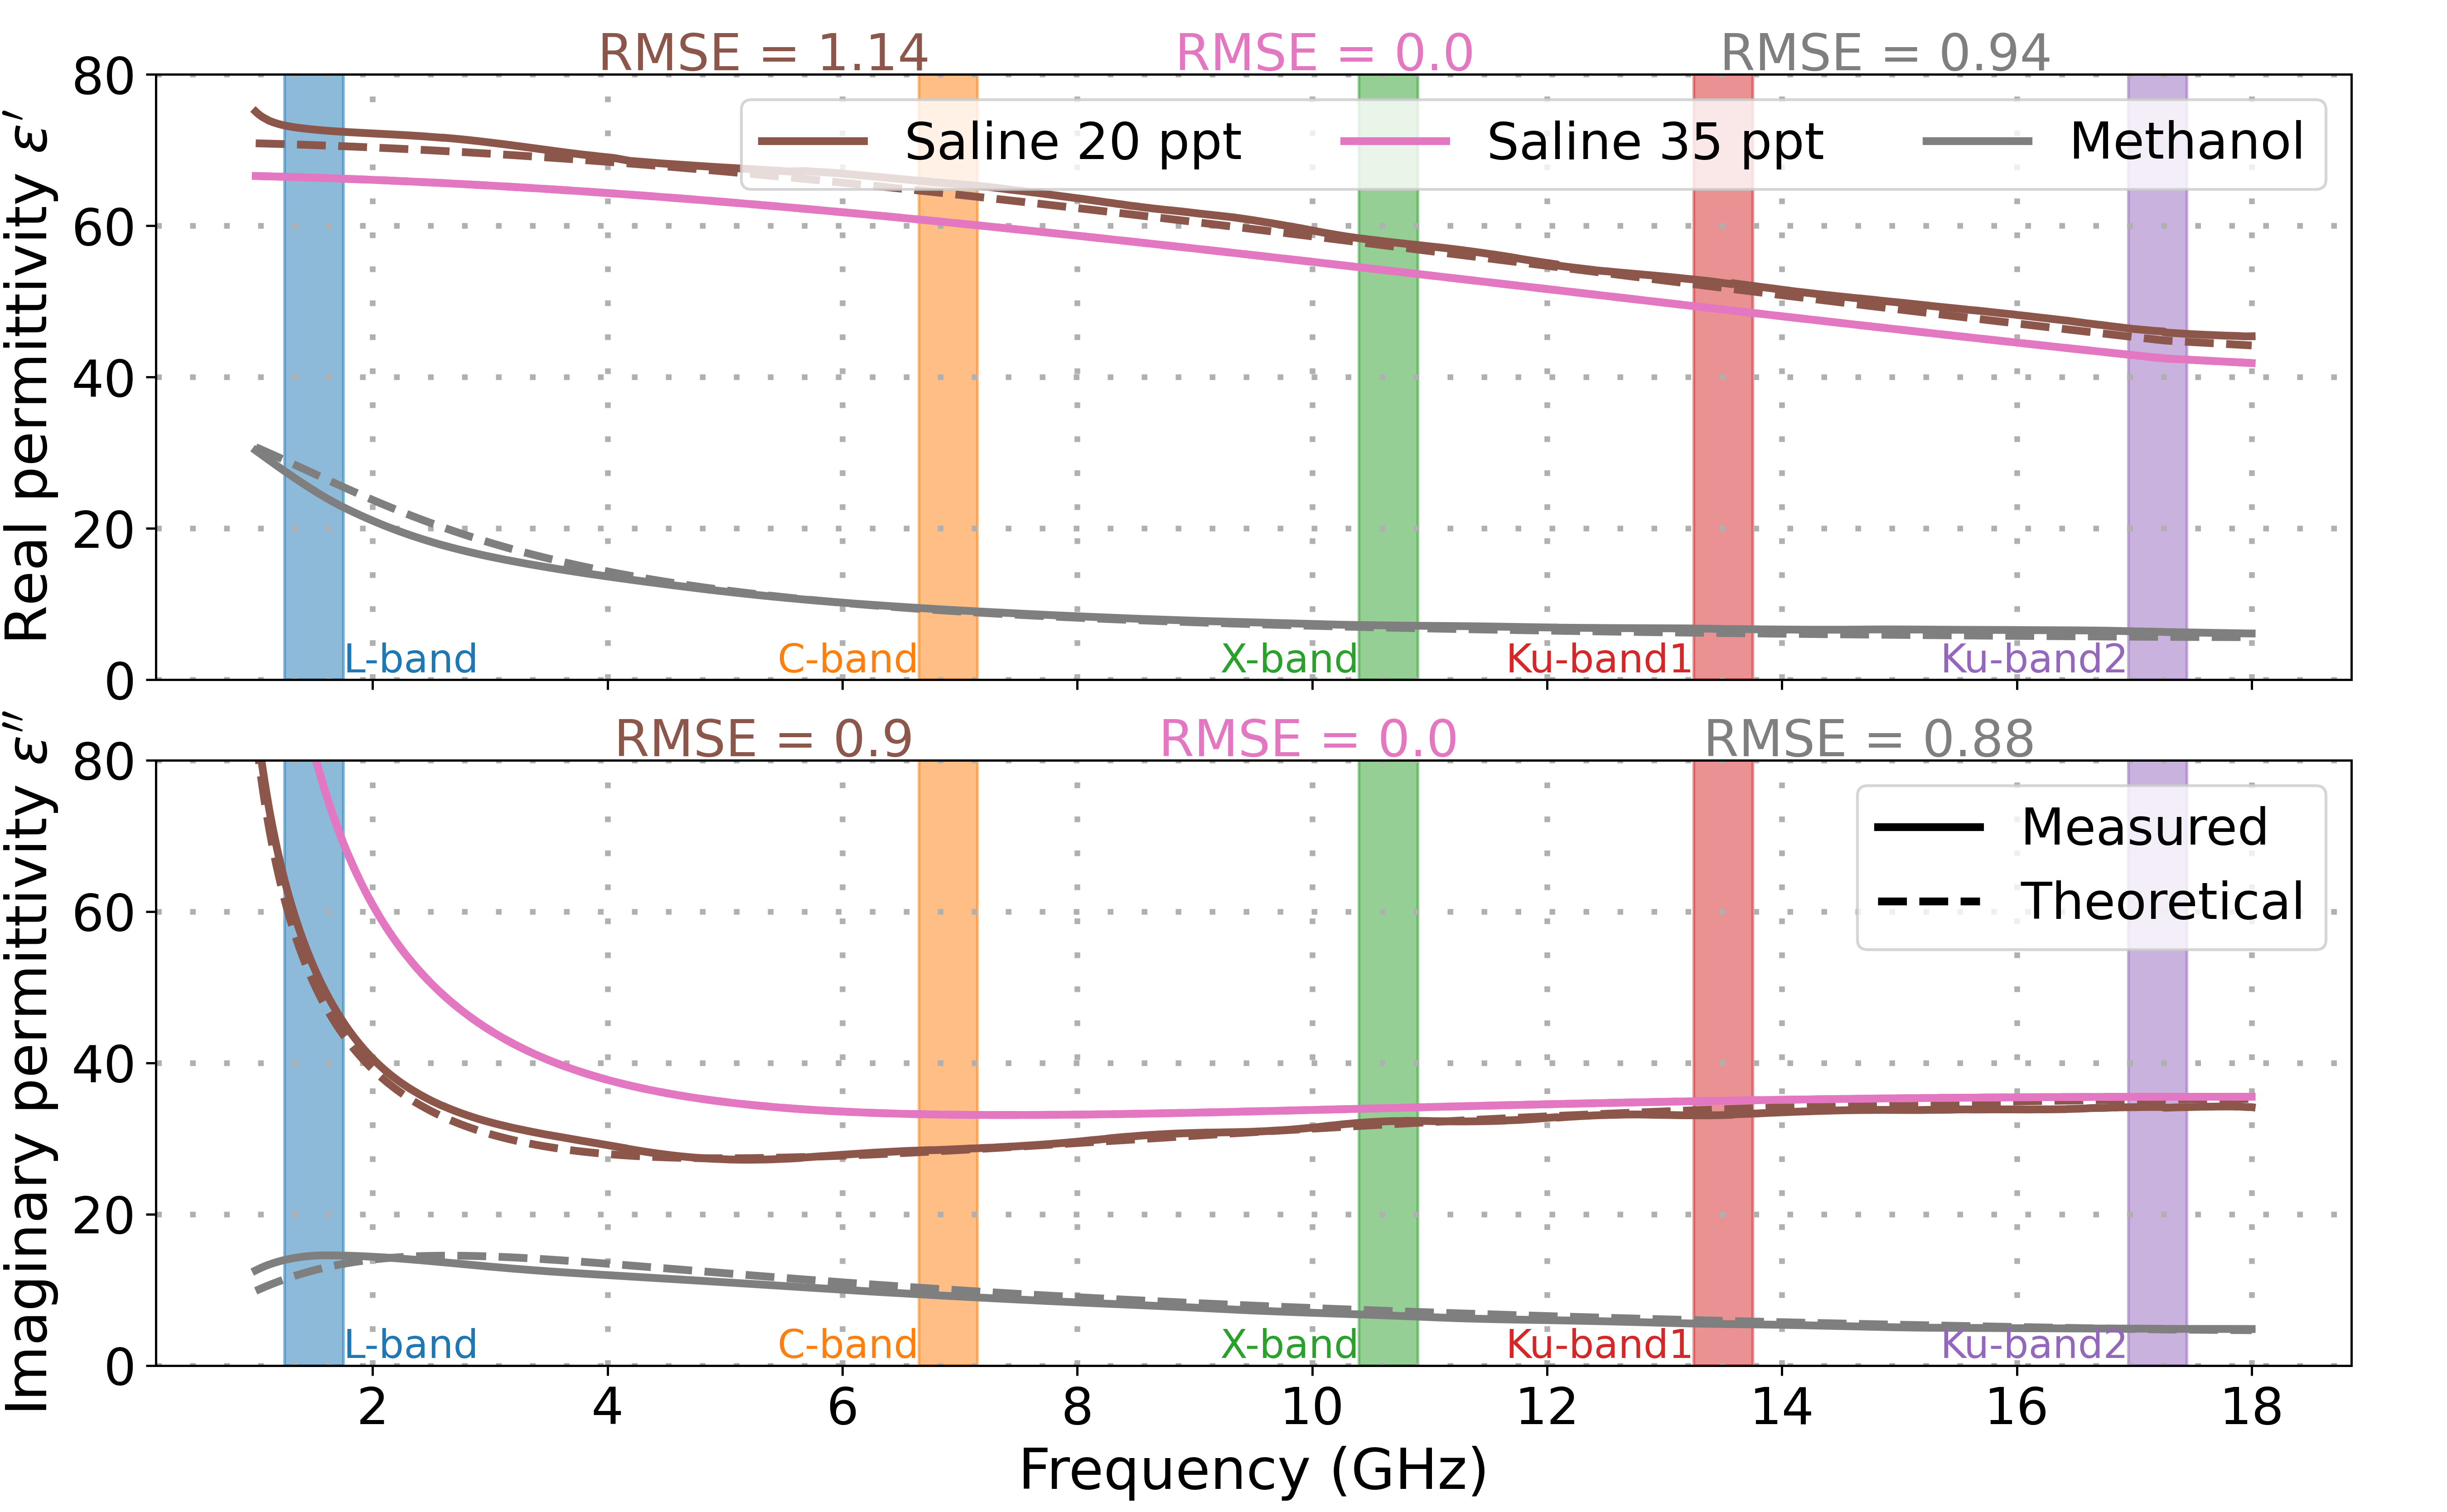
\includegraphics[width=\columnwidth]{Images/calibration-results.png}
    \caption[]{Theoretical and measured permittivity of saline solution and methanol with their associated \ac{rmse}. The selected relevant frequency ranges for remote sensing applications were also highlighted}\label{fig:calib-results}
\end{figure}

\subsection{Signal penetration depth}

\begin{figure}[ht!]
    \centering
    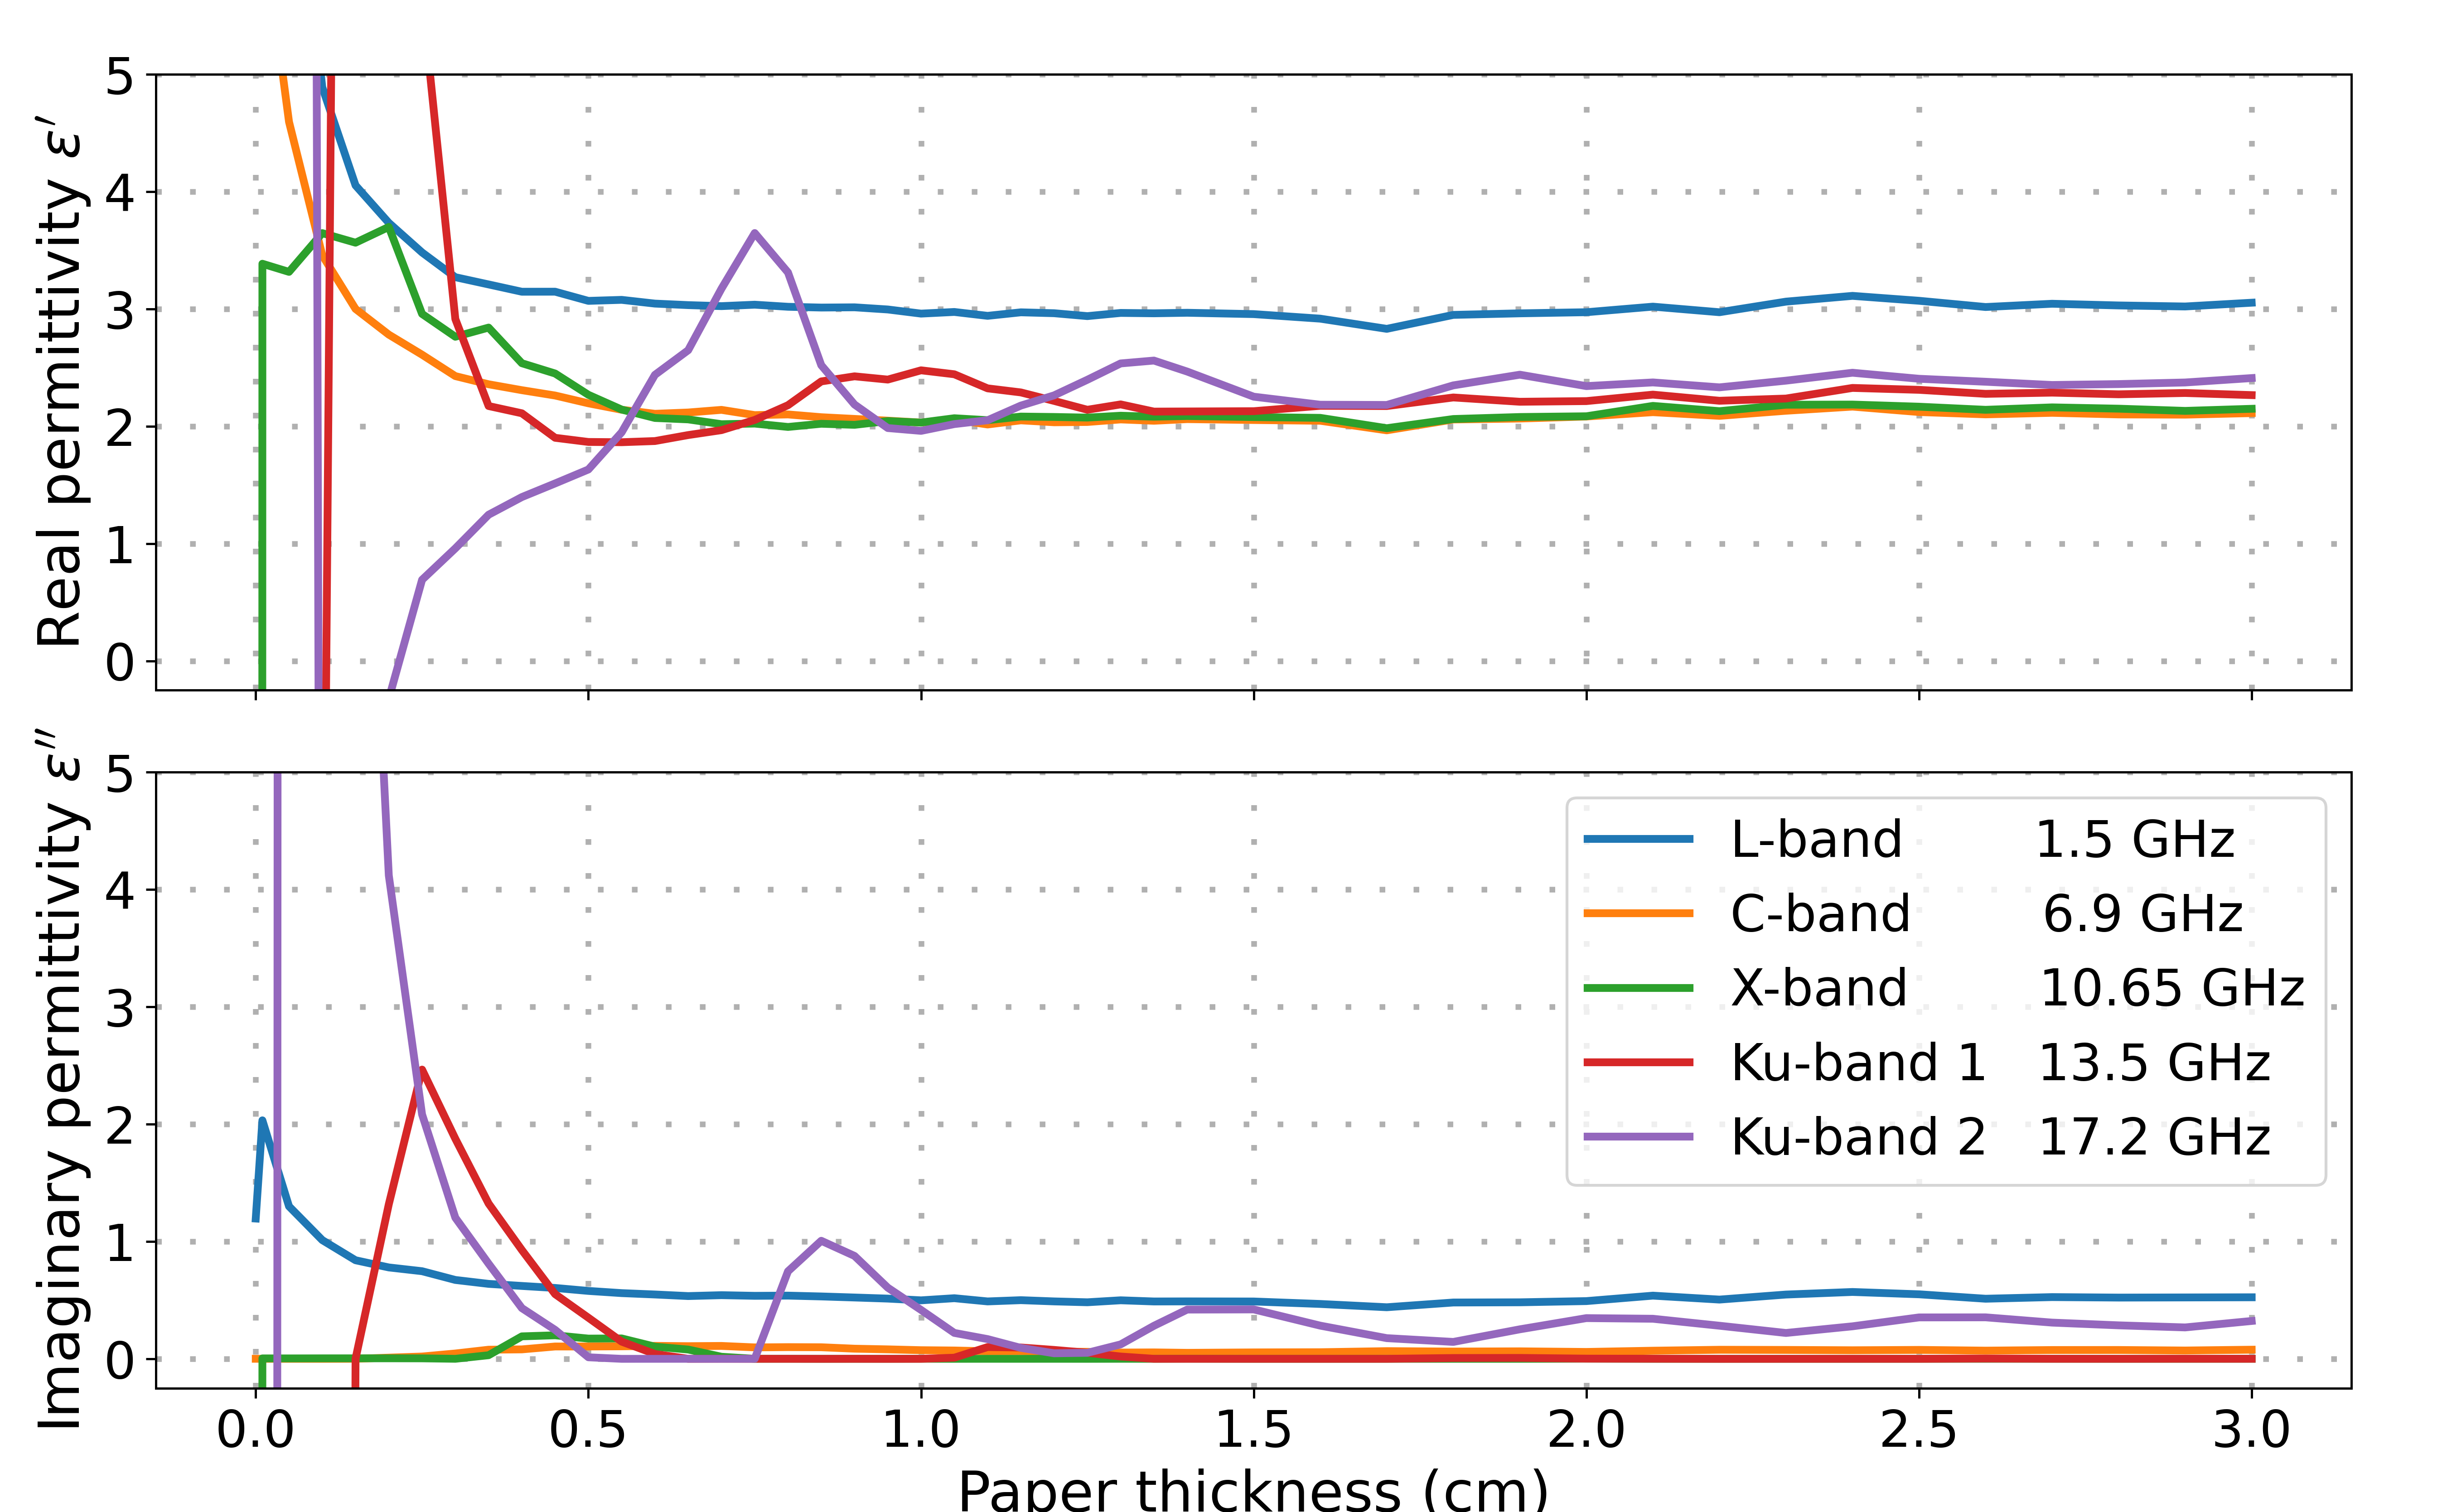
\includegraphics[width=\columnwidth]{Images/dry-paper.png}
    \caption[]{Estimation of the probe signal penetration depth on dried paper for relevant frequencies}\label{fig:dry-paper}
\end{figure}

For dry paper, at L-band (\qty{1.4}{\giga\hertz}), the curve stabilized around \qty{0.5}{\cm} for a value of \(\varepsilon^\prime = 3\) which is coherent with \parencite{Elrayes1987} who found a value around \(\varepsilon^\prime\approx2.9\) at \qty{1}{\giga\hertz}.
Figure~\ref{fig:dry-paper} also shows that the probe signal stabilizes around \qty{0.75}{\cm} for the other bands.
Considering that the outer diameter of the probe is of \qty{13.2}{\mm}, the results are consistent with the rule of thumb proposed by \textcite{Elrayes1987} that the probe penetration depth in a low loss material such as paper is approximately equal to the inside diameter of the outer conducting cylinder of the probe (see left side of figure~\ref{fig:probe-scheme}, measurement 2b = \qty{13.2}{\mm}).

% Measurements using the OECP are only based on the transient (not radiated) wave whose propagation is limited throughout the close volume of the material at the contact surface with the OECP’s aperture.
% However, slight amount of radiation waves also propagate through the material, reflect against the sample edges, then may get back to the probe, causing so measurements errors. This is the reason why the saline solution containers are chosen to be sufficiently large to allow waves damping and avoid radiation reflections.
% In thin materials, radiations are more likely to reflect into the probe. To reduce this effect, it is important to work with greater wavelengths where the probe’s radiation is neglectable. This can be achieved by using low permittivity dielectrics (like paper) and working at lower frequencies. However, at higher frequencies where the wavelength is reduced and gets closer to the OECP’s cross section, it becomes impossible to prevent radiative waves effect.
% The only allowable option is to rely on the result obtained at lower frequencies. This is justified by the fact that the obtained depth is relatively constant for all the frequencies up to the X-Band. Moreover, when the paper is wet, which causes damping, the result is the same for all the frequencies without exception. Damping has prevented radiative waves, but has also reduced the extent of the transient wave, which is why the dry paper result at low frequency is estimated to be the most reliable.
% For the measurement made during this work, the samples a sufficiently thick (more than 10cm) to avoid the radiation effect for the materials’ permittivity range.


\begin{figure}[ht!]
    \centering  
    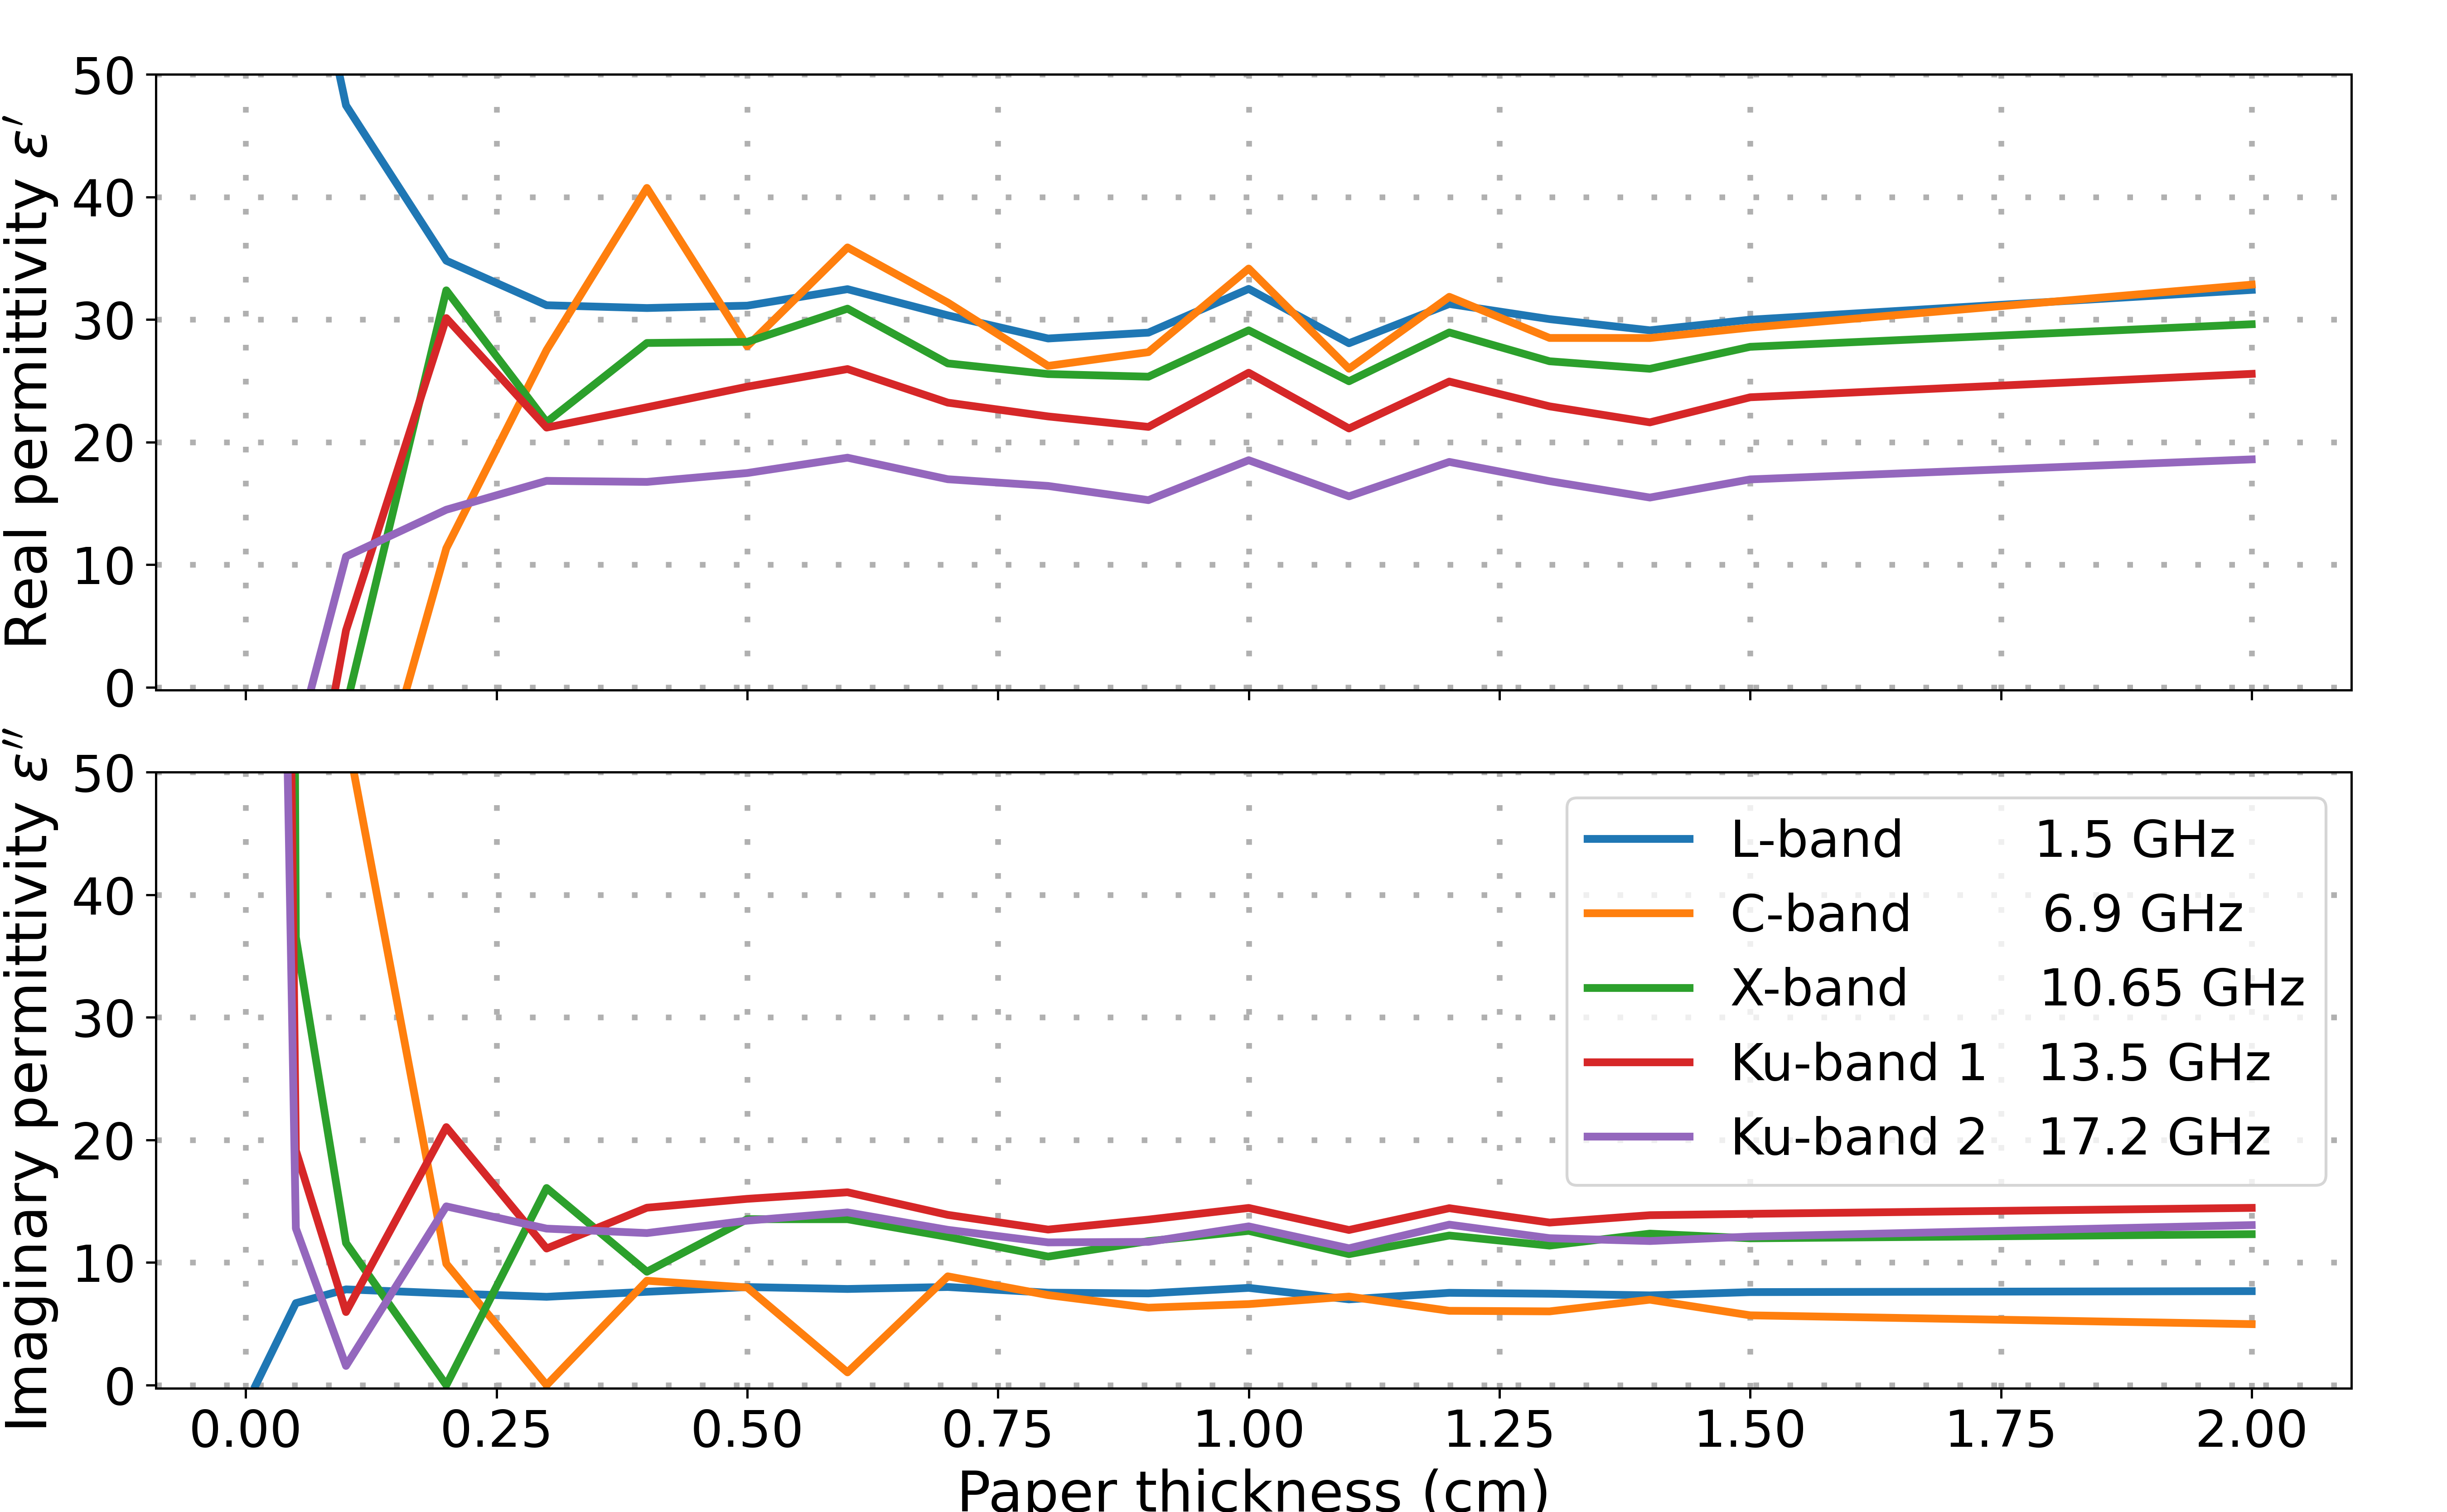
\includegraphics[width=\columnwidth]{Images/wet-paper.png}
    \caption[]{Estimation of the probe signal penetration depth on soaked paper for relevant frequencies}\label{fig:wet-paper}
\end{figure}

Figure~\ref{fig:wet-paper} results for wet paper are interpreted similarly.
However, since the paper's water content increases the dielectric loss, the real permittivity decreases for higher frequencies.
The signal loss from the conducting copper plate noticeably happens with fewer stacked sheets than with dry paper.
The probe's penetration depth in higher loss material can be estimated at around \qty{0.3}{\cm}.
Another noticeable difference between dry and wet paper comes from the oscillations with both Ku-band frequencies between \qtyrange{0.5}{1.5}{\cm} for dry paper.
These oscillations result from noise created by unwanted reflection in the dry paper medium.
Indeed, the probe signal in a medium such as dry paper at high frequencies, where the wavelengths are closer in scale to the \ac{oecp} cross-section, is more likely to be reflected on the sample edge and cause unwanted fluctuations in the reflection readings.
At frequencies closer to L-band and C-band, where the wavelengths are larger, such unwanted reflections are negligible.
In liquids such as the saline solutions used in the probe calibration process or in a moist medium such as wet paper, the probe signal is damped, preventing unwanted reflections.
This signal damping also causes the penetration depth to be equal across all frequencies in the wet medium. 
These penetration depths mean that, to safely measure only the desired sample and not its container, a safe minimal soil depth would be over \qty{2}{\cm}.
In the present study, the soil sample used are well over this limit with a \qty{10}{\cm} depth.

% See table~\ref{tab:dry-wet-paper} for a summary of the penetration depths.
% \begin{table}[ht!]
%     \centering
%     \caption{Penetration depth (cm) at different frequency in dry and wet paper sheet stacks}\label{tab:dry-wet-paper}
%     \begin{tabular}{r l c c c c}
%         Medium & L-band & C-band & X-band & Ku-band 1 & Ku-band 2 \\
%         \midrule\midrule
%         Dry paper & 0.5 & 0.75 & 0.75 & 1.25 & 1.5 \\
%         Wet paper & 0.3 & 0.3  & 0.3  & 0.3  & 0.3 \\
%     \end{tabular}
% \end{table}

% These results may seem contradictory, where usually, with constant permittivity, the penetration depth would decrease with the frequency.
% In our case, the opposite happens since water permittivity decreases with frequency

\subsection{Dry sand spectrum}
Since the dry sand permittivity does not vary in this range of temperature, its real and imaginary permittivity are compared to literature data from \textcite{Matzler1998} (see Figure~\ref{fig:dry-sand}).
In \parencite{Matzler1998}, the permittivity of dry sand gathered in the Sahara Desert in the frequency range of \qtyrange{0.245}{6}{\giga\hertz} was found to be around \(\varepsilon = 2.6 - \left[0.13, 0.012\right]j\).

\begin{figure}[ht!]
    \centering
    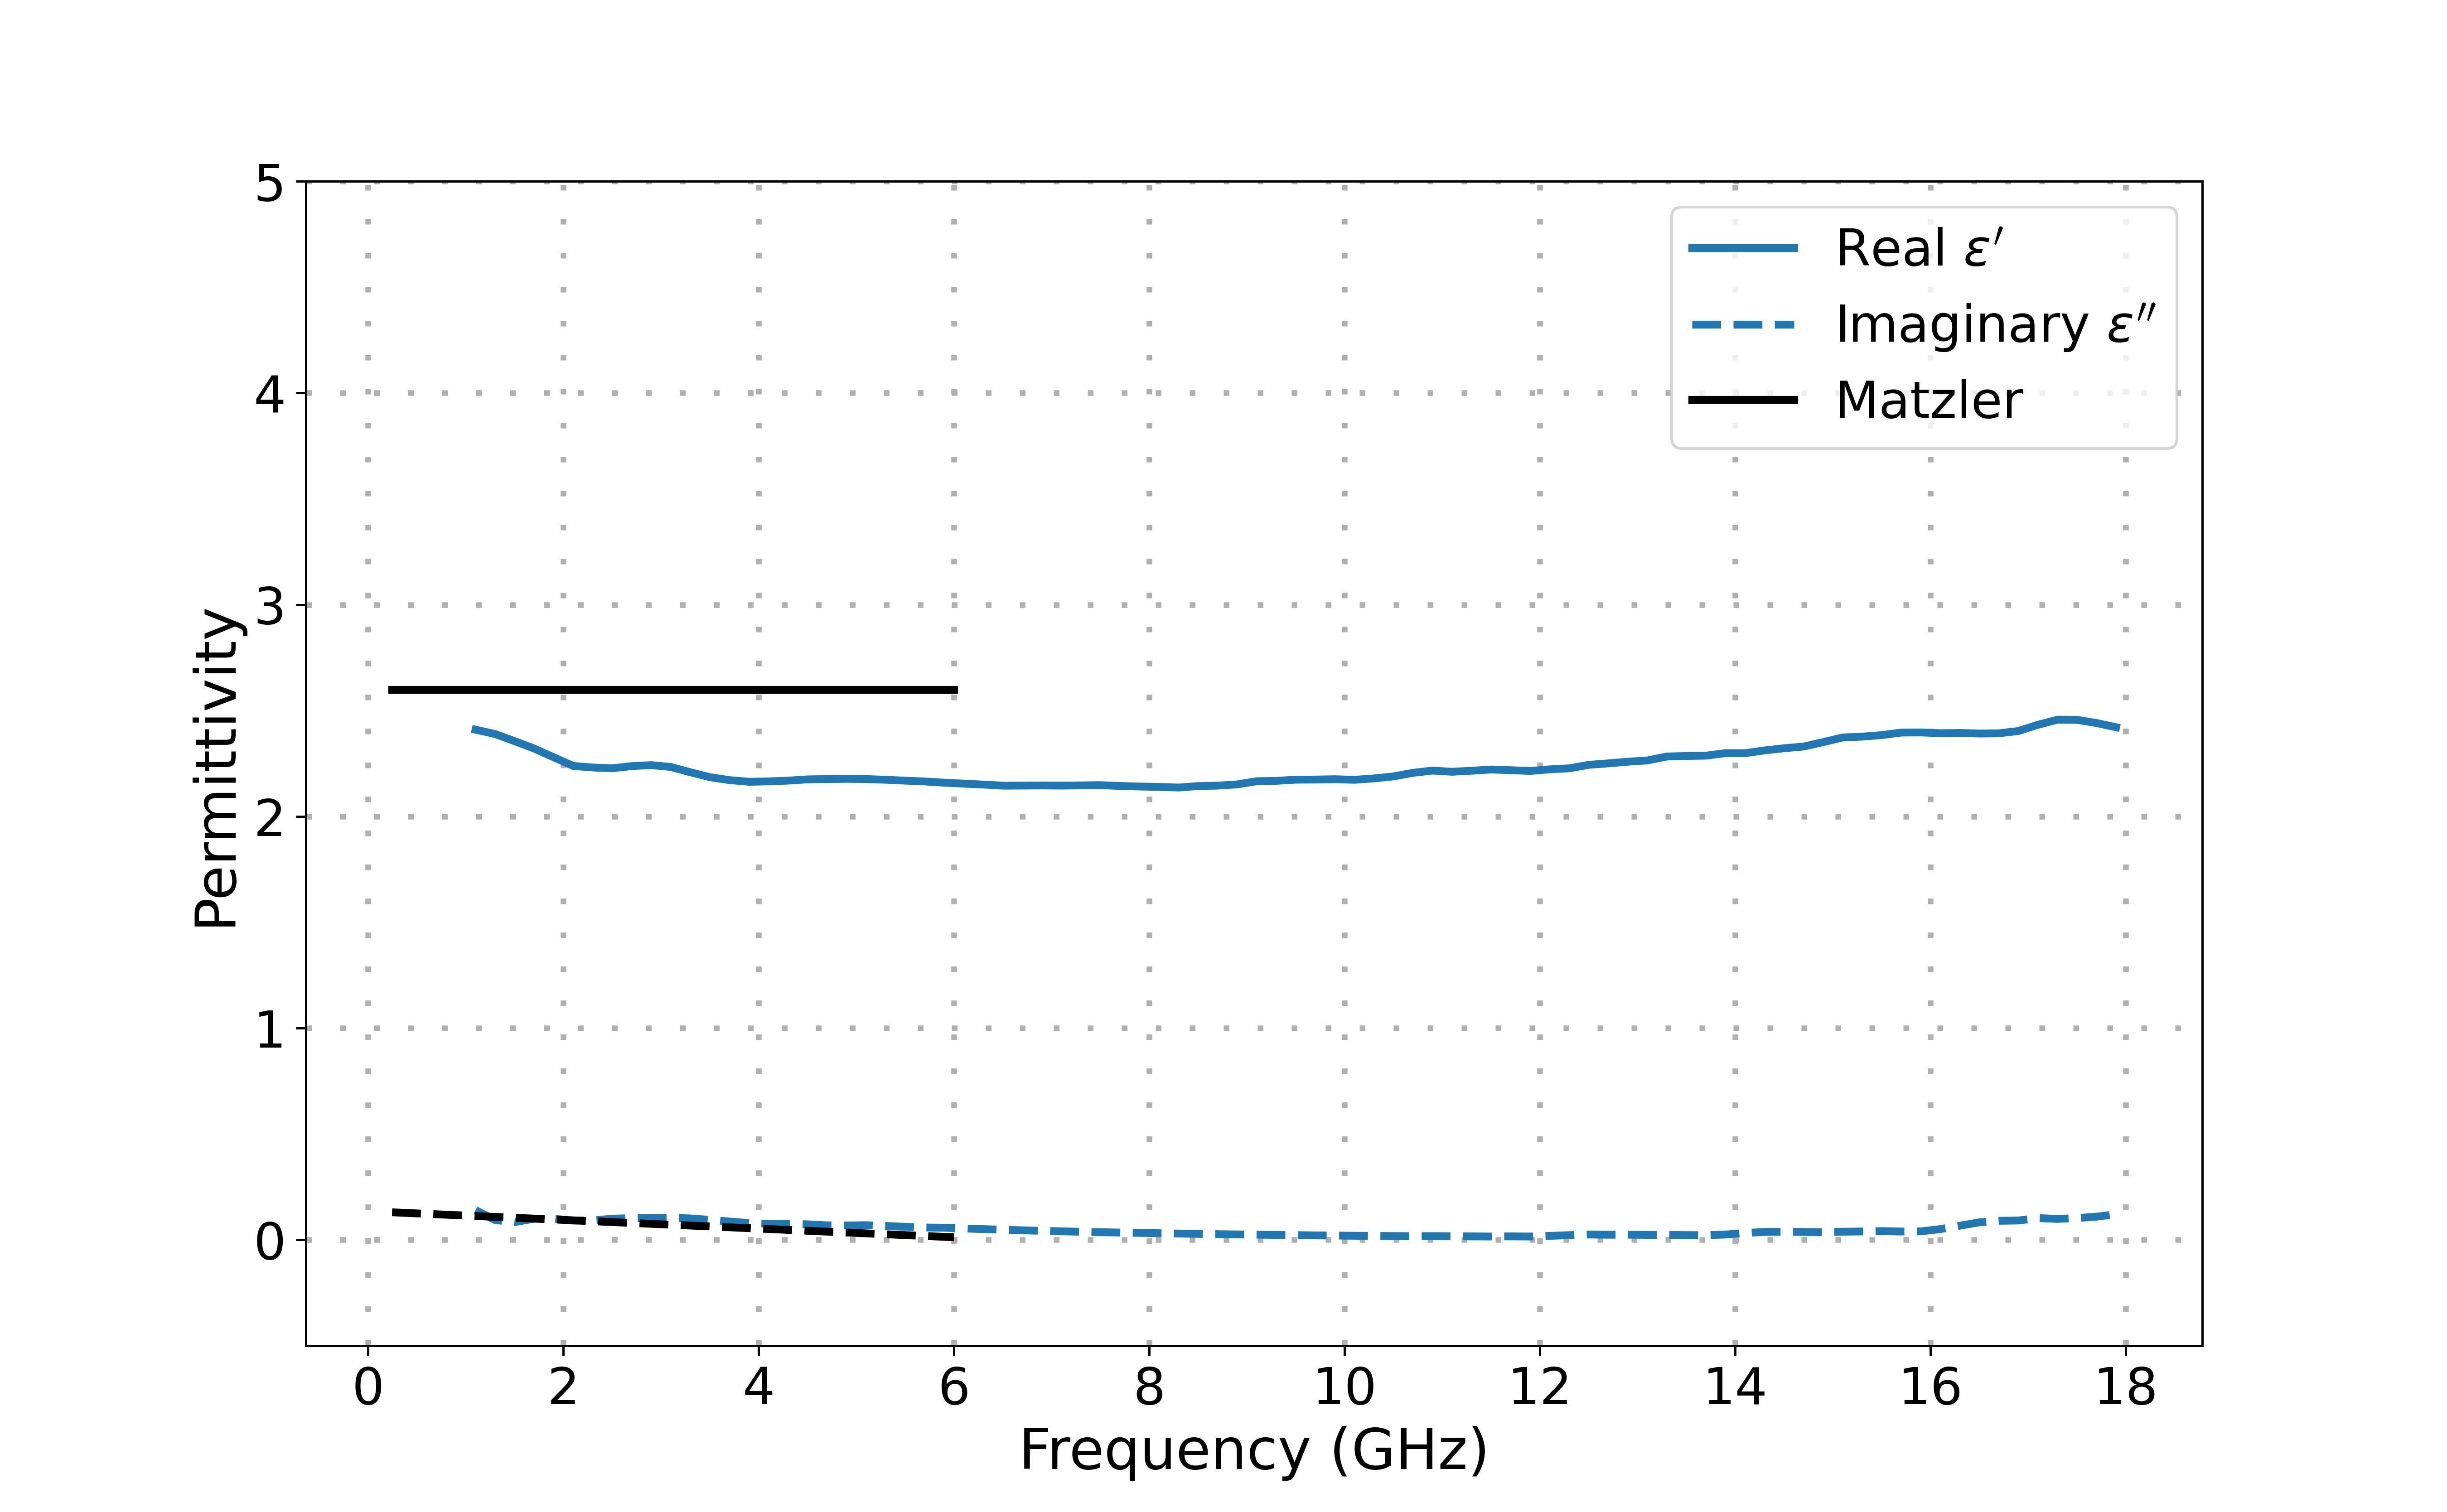
\includegraphics[width=\columnwidth]{Images/dry-sand.png}
    \caption[]{Measurement of dry sand permittivity on all available frequencies compared to the measurements from \textcite{Matzler1998}}\label{fig:dry-sand}
\end{figure}

Figure~\ref{fig:dry-sand} shows that the result obtained from the probe used in the present study are consistent with what was found in the literature with a real permittivity slightly above \(\varepsilon^\prime = 2\) at lower frequencies and around \(\varepsilon^\prime = 2.6\) at the higher end.
However, the permittivity presented in this paper is below the one from \textcite{Matzler1998} in their study range of \qtyrange{0.245}{6}{\giga\hertz}.
This can be explained by the grain size or physical properties of the sand \parencite{Schmugge1980}.
Indeed, varying the density would change the permittivity, where a denser sample would have a higher permittivity since less air (\(\varepsilon^\prime = 1\)) is present in the analyzed volume. 

\subsection{Freezing cycle on wet sand and organic soil}

\begin{figure}[ht!]
    \centering
    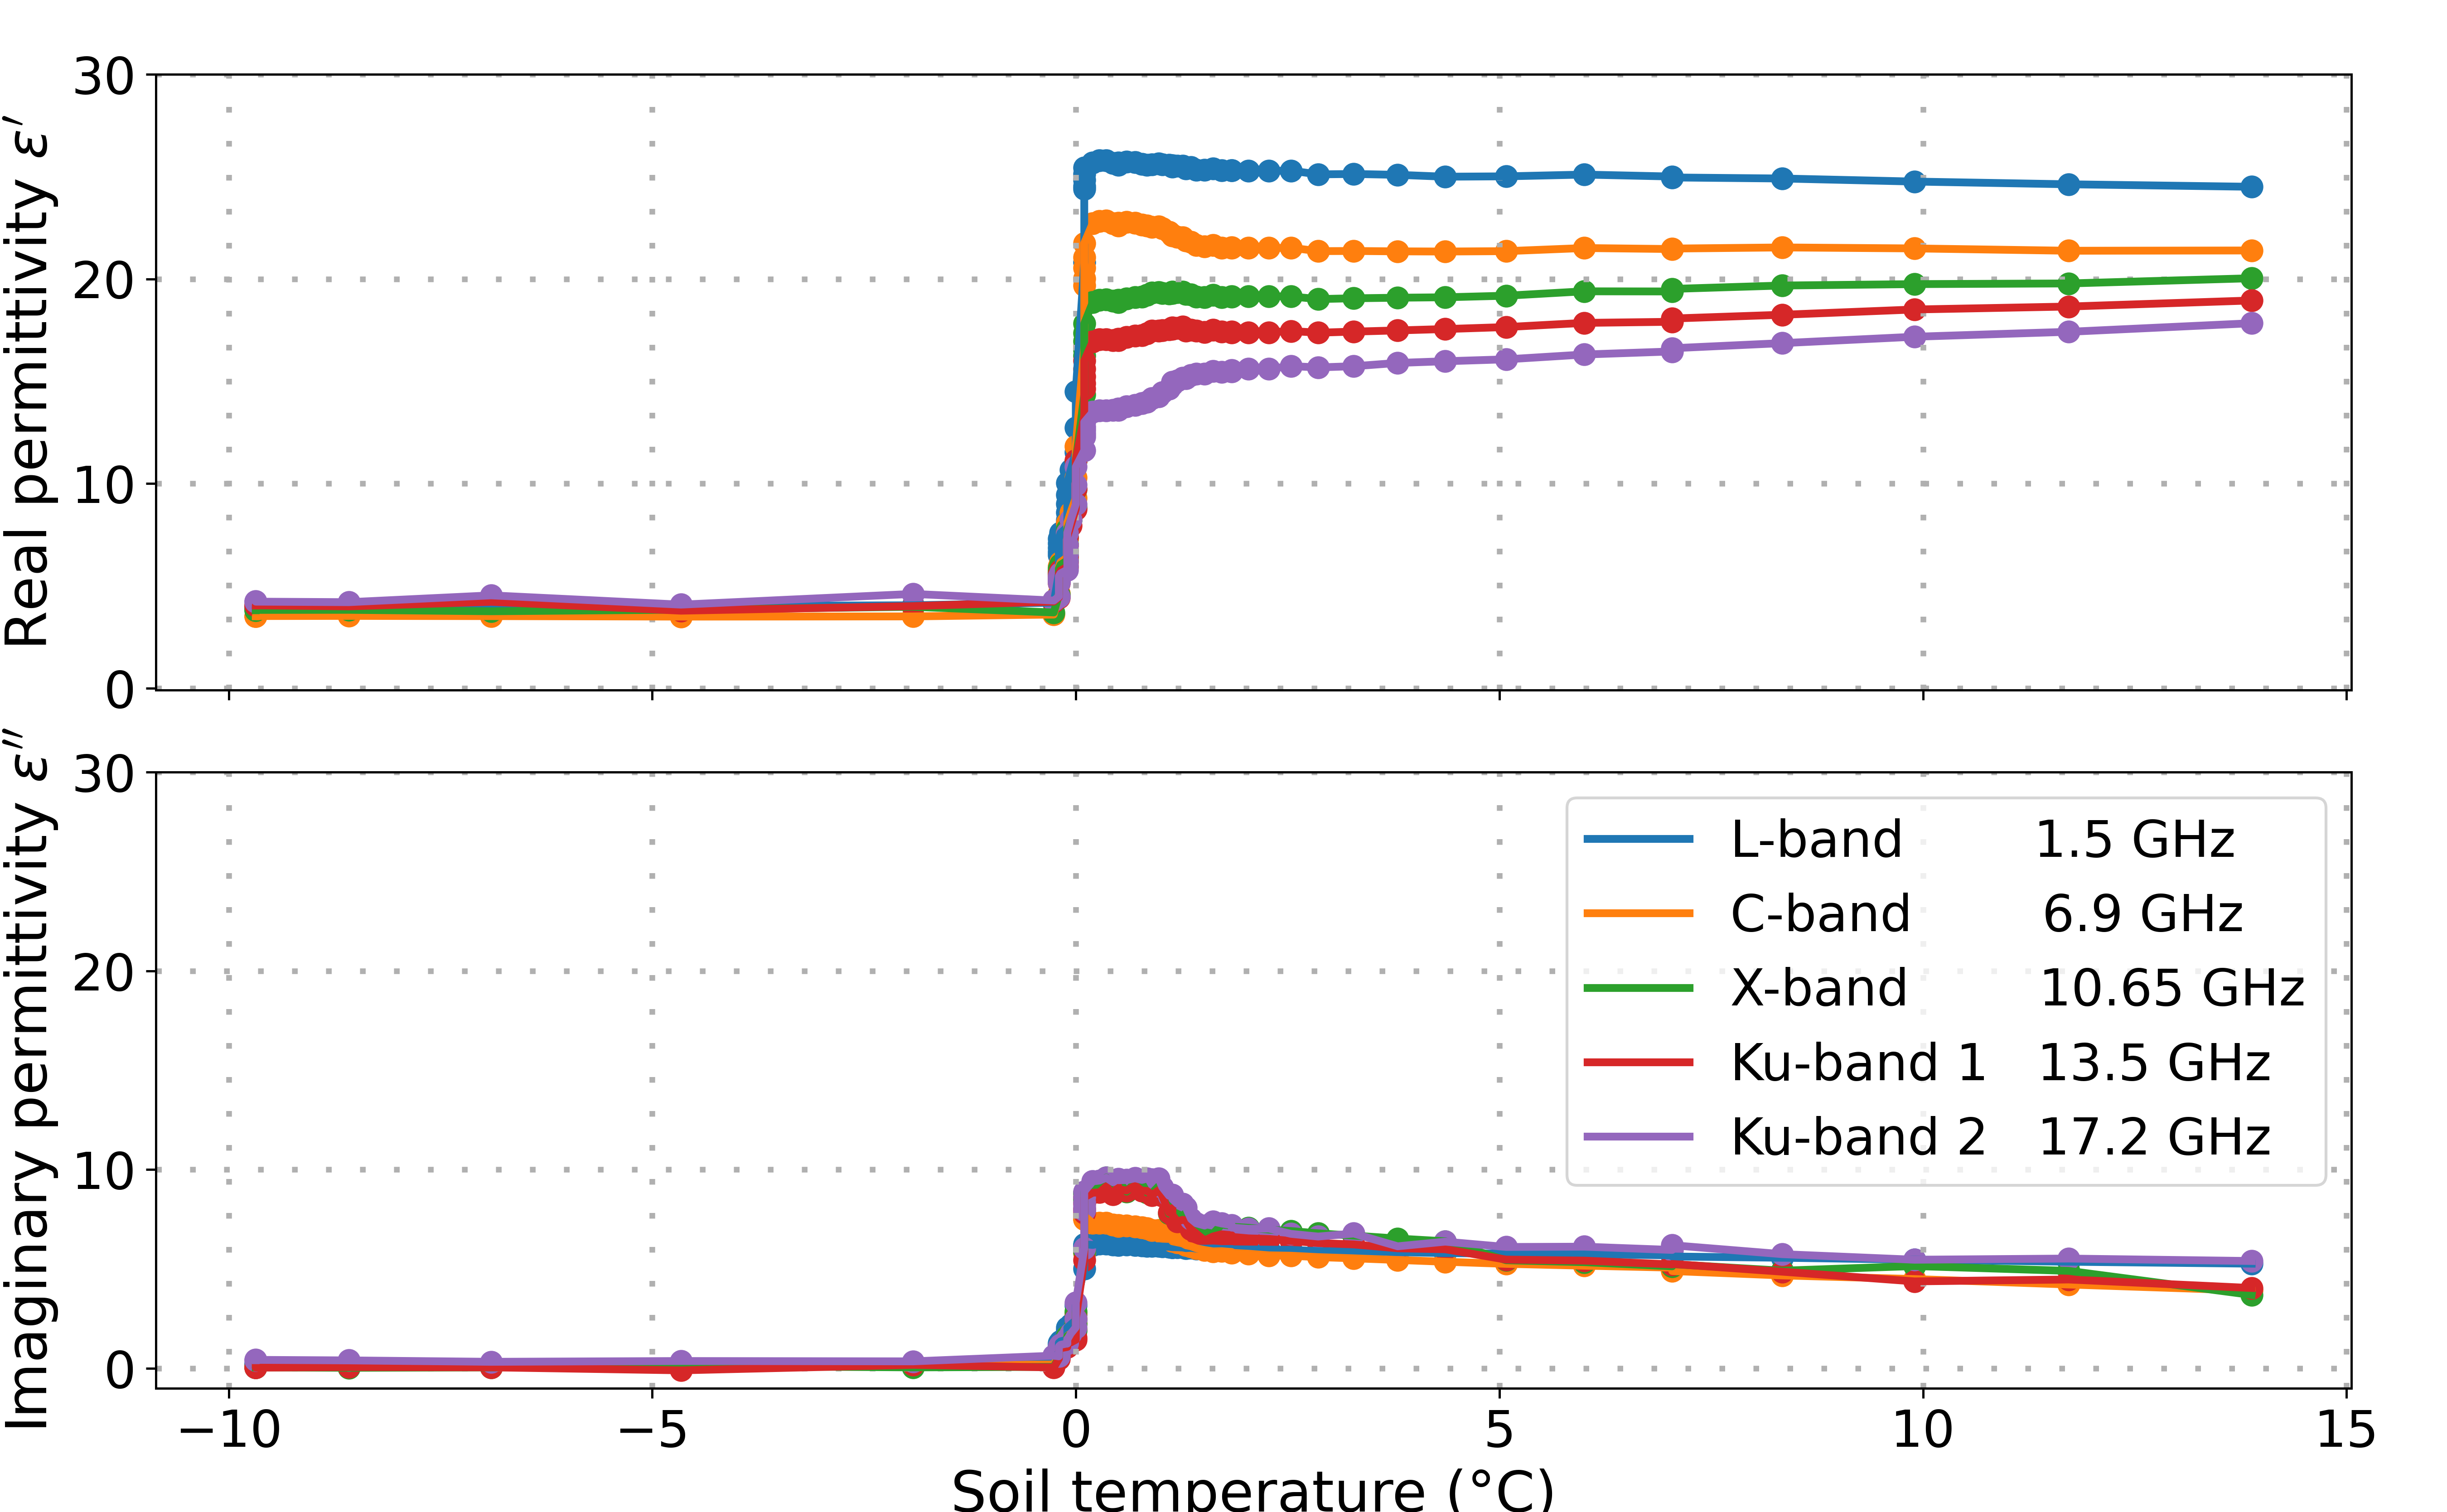
\includegraphics[width=\columnwidth]{Images/wet-sand.png}
    \caption[]{Freeze/thaw cycle of sand with 25\% w/w relative humidity}\label{fig:wet-sand}
\end{figure}

Figure~\ref{fig:wet-sand} shows results of the temperature cycle on the \qty{25}{\percent} weight/weight relative humidity sand.
The graph shows that above \qty{0}{\degreeCelsius}, the permittivity decreases with increasing frequency due to the sand water content, matching what was previously observed for the wet paper (Figure~\ref{fig:wet-paper}).
There also seems to be a slight temperature dependency for the Ku-1- and Ku-2- bands where the permittivity increases as temperature rises.
This increase is due to the variation of the water permittivity as a function of temperature \parencite{Kaatze1989}.
At temperatures lower than \qty{0}{\degreeCelsius}, a sharp decrease in permittivity followed by a plateau is observed, where all frequencies are approximately at the same value (around \(\varepsilon^\prime = 5\)).

\begin{figure}[ht!]
    \centering
    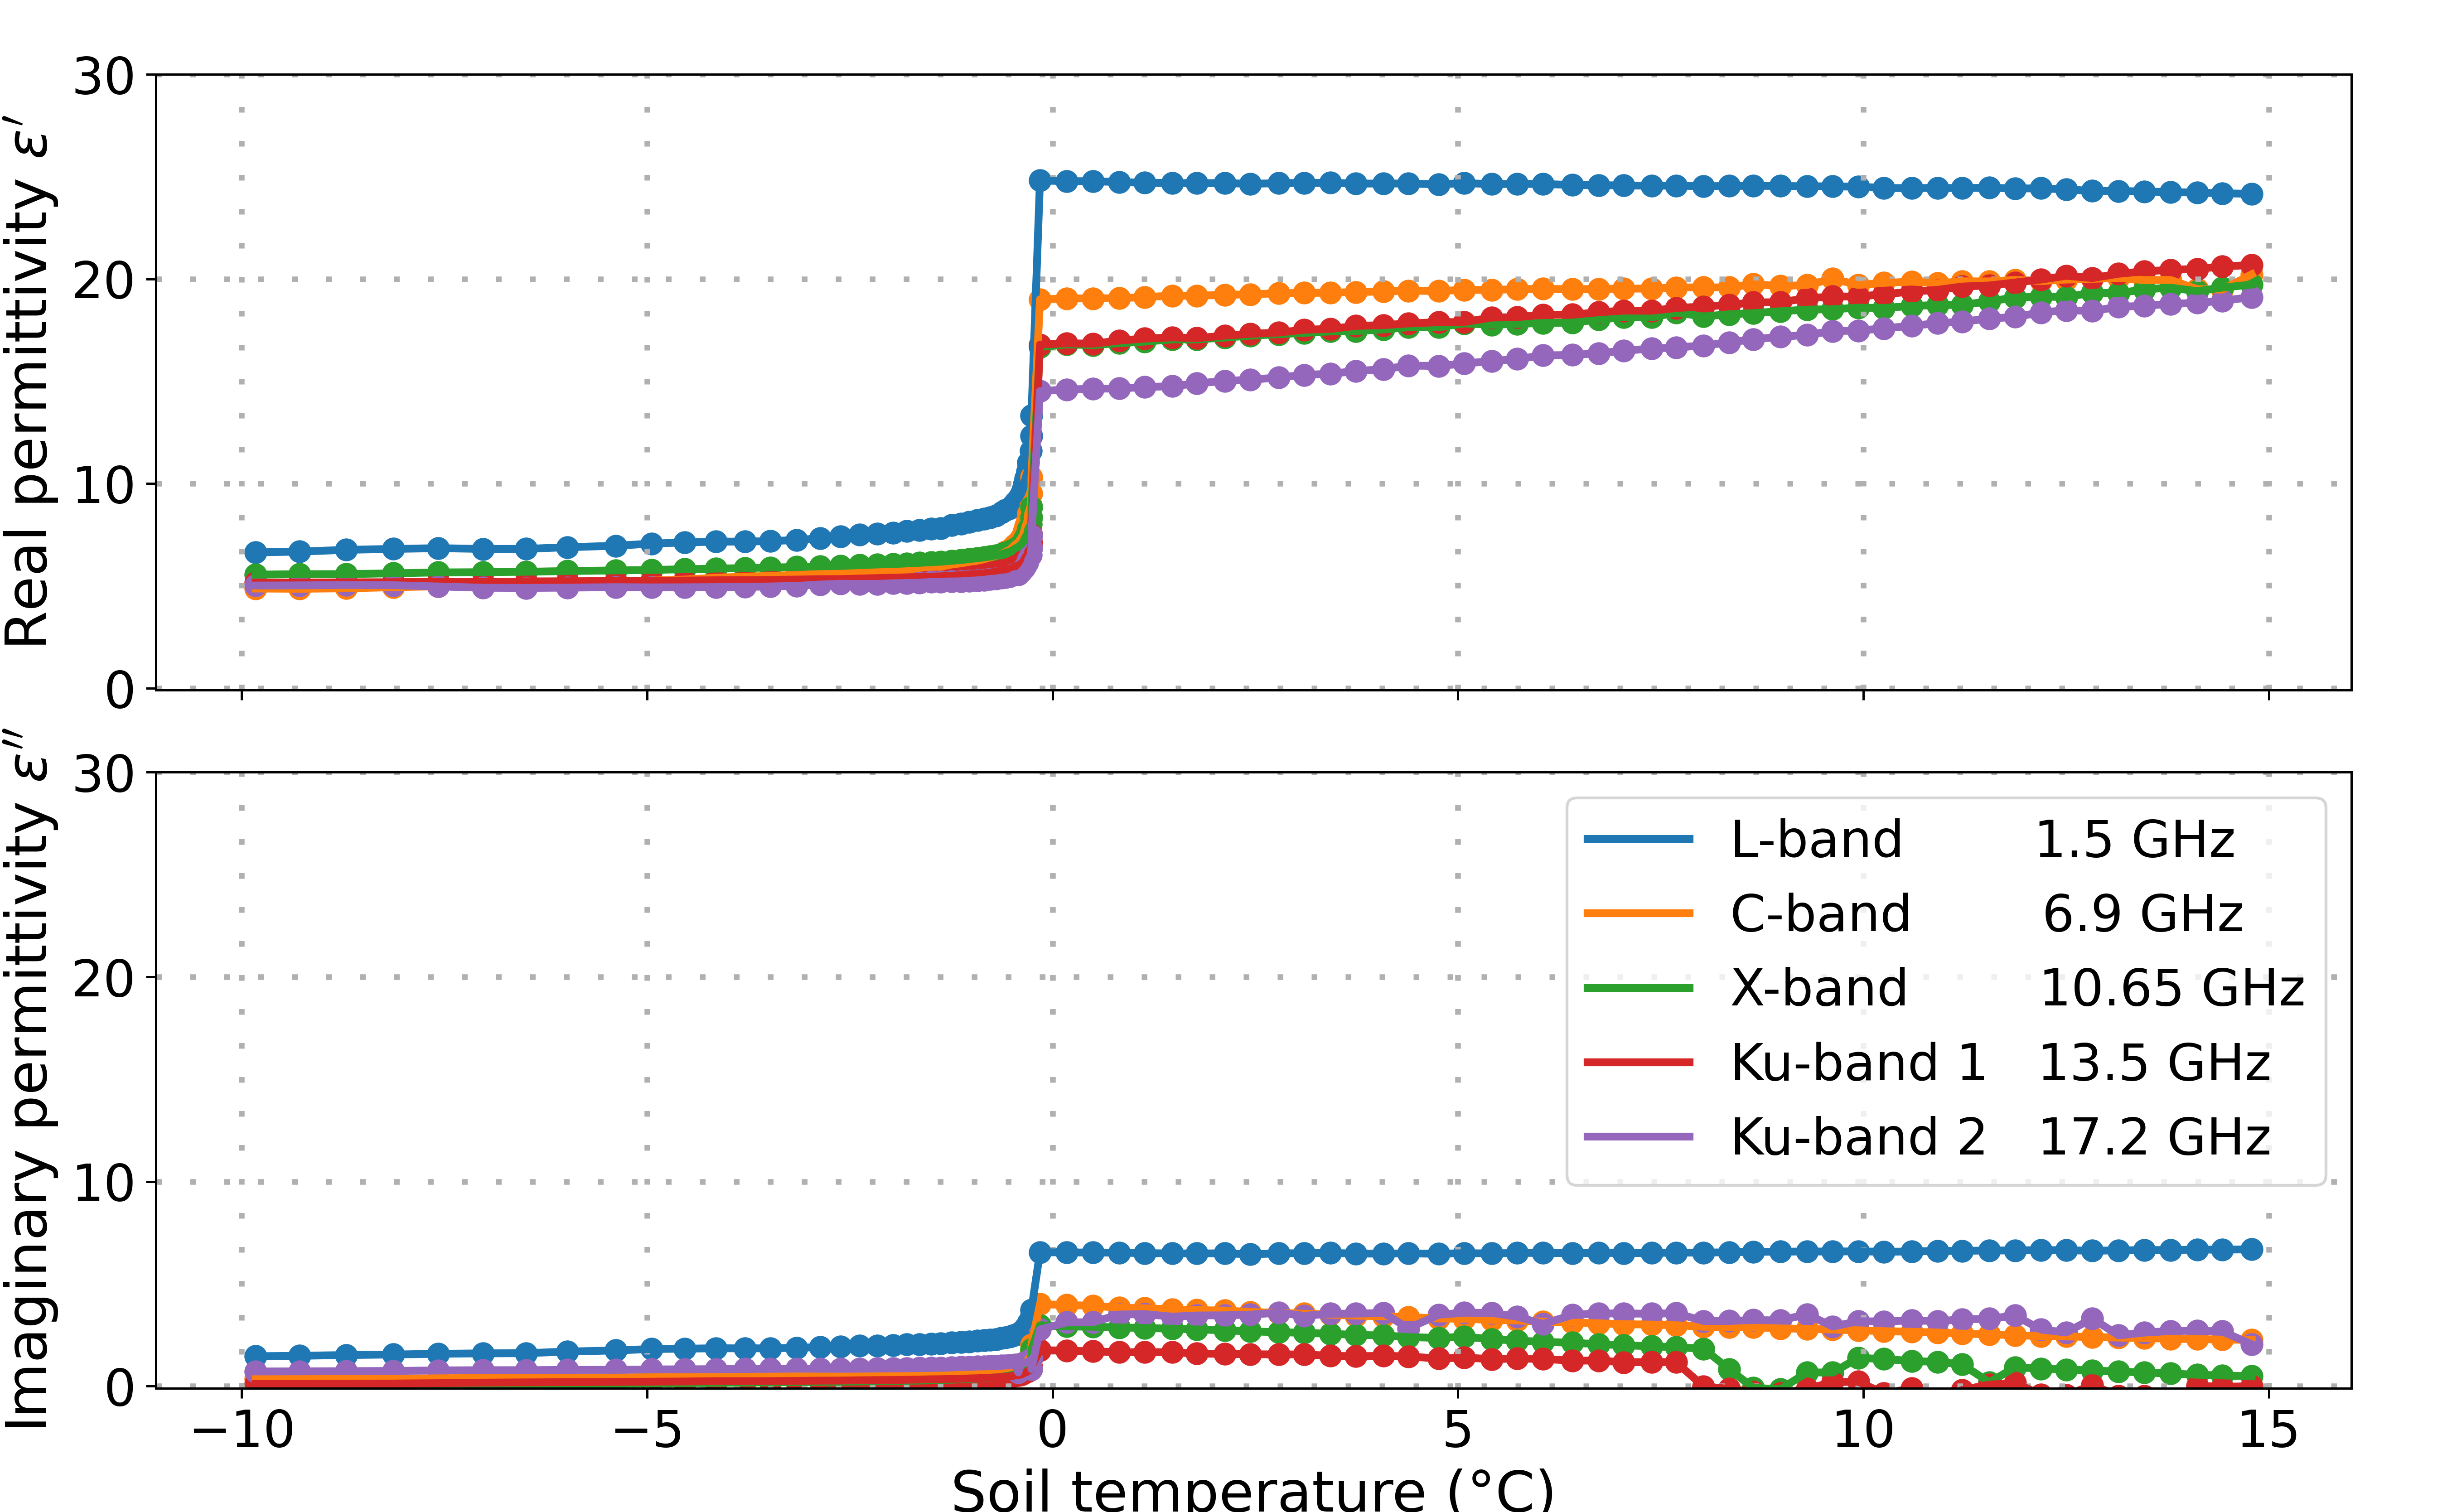
\includegraphics[width=\columnwidth]{Images/wet-soil.png}
    \caption[]{Freeze/thaw cycle of wet organic mesic soil}\label{fig:wet-soil}
\end{figure}

Figure~\ref{fig:wet-soil} shows the permittivity for an arctic organic soil sample (Cambridge Bay).
This sample also seems to show a greater temperature dependency above \qty{0}{\degreeCelsius} for the X- and both Ku-bands than the commercial sand where the permittivity increases with the temperature.
At \qty{15}{\degreeCelsius}, the permittivity of the organic soil sample for the multiple highlighted frequencies converges around \(\varepsilon^\prime = 20\), while the sand sample permittivity is more spread at the same temperature.
The below \qty{0}{\degreeCelsius} permittivity also drops sharply, then plateaus when the water inside the sample is completely frozen at a value around \(\varepsilon^\prime = 5\), like the commercial sand.

Table~\ref{tab:mean-eps} shows the average real permittivity of each plateau when the sample is either completely frozen or completely thawed.
The uncertainty on the numbers presented in the table comes from a standard deviation from the average.
The presented values can be used to parametrize radiative transfer models to compute brightness temperature or backscattering coefficients for remote sensing applications.

\begin{table}[ht!]
\centering
\caption{Mean real permittivity of the frozen (T\(\leq\)\qty{-0.5}{\degreeCelsius}) and thawed (T\(\geq\)\qty{0.5}{\degreeCelsius}) sample for each relevant band frequencies}\label{tab:mean-eps}%
\resizebox{\columnwidth}{!}{%
\begin{tabular}{l c c c c}
    & \multicolumn{2}{c}{Wet sand} & \multicolumn{2}{c}{Organic soil} \\
    & Frozen & Thawed & Frozen & Thawed \\
    \midrule\midrule
    L-band (\SI{1.5}{\giga\hertz})   & \(4.03\pm0.04\) & \(25.3\pm0.2\) &
                                       \(7.6\pm0.6\) & \(24\pm2\) \\
    C-band (\SI{6.9}{\giga\hertz})   & \(3.52\pm0.02\) & \(21.7\pm0.3\) & 
                                       \(5.8\pm0.5\) & \(19\pm2\) \\
    X-band (\SI{10.65}{\giga\hertz}) & \(3.85\pm0.09\) & \(19.2\pm0.2\) & 
                                       \(6.1\pm0.3\) & \(17\pm2\) \\
    Ku-band 1 (\SI{13.5}{\giga\hertz})    & \(4.1\pm0.2\) & \(17.5\pm0.2\) & 
                                            \(5.4\pm0.2\) & \(17\pm2\) \\
    Ku-band 2 (\SI{17.2}{\giga\hertz})    & \(4.3\pm0.2\) & \(15.5\pm0.5\) & 
                                            \(5.1\pm0.2\) & \(15\pm2\) \\
\end{tabular}}
\end{table}

\subsection{Potential applications for satellite missions}
Our unique \acl{oecp} has a large aperture allowing repeatable and precise permittivity measurements of heterogeneous materials while having a frequency band ranging from \qtyrange{0.5}{18}{\giga\hertz}.
The permittivity measurements of the wet commercial sand and of the arctic organic soil sample presented in this work vary greatly whether the soil is frozen or unfrozen, and between the highlighted frequency bands above \qty{0}{\degreeCelsius}.
This has a special importance for \ac{tsmm}, where the soil effect on the snow water equivalent inversion from Ku-band \ac{sar} is still misunderstood \parencite{King2018,Rutter2019}.
Furthermore, at Ku-band, the possible variability of the frozen soil permittivity due to the soil texture and composition, especially for arctic organic soil, is undetermined.
Some studies also show the effect of the zero-curtain \parencite{Outcalt1990,Domine2018} in arctic and boreal forest soils, where the soil under a snowpack is not completely frozen, which can greatly influence the permittivity, hence the backscattering signal.

To follow up this calibration and characterization work with the \ac{oecp}, we plan on applying the freezing/thawing protocol presented above to an array of soil from different places to analyze the permittivity as a function of the soil texture, organic matter percentage, temperature and humidity.
The database created with these soil characterization will then be used to produce a wideband permittivity model spanning the whole probe range.

\section{Conclusion}
In this paper, we presented a novel \acl{oecp} that can measure the permittivity of a heterogeneous sample over a large frequency band (\qtyrange{0.5}{18}{\giga\hertz}), which is especially relevant for microwave remote sensing.
Here, we chose to only present the results for relevant satellite-based remote sensing sensor frequencies that are commonly used for snow monitoring.
The probe calibration shows its reliability over all the \qtyrange{0.5}{18}{\giga\hertz} range with minimal errors (RMSE \(\approx1\)).
Tests on dry and wet stacked paper were used to determine that the penetration depth of the probe signal is between \qtyrange{0.5}{0.75}{\cm} depending on the frequency for the dry paper and around \qty{0.3}{\cm} for wet paper.
The probe was also used to measure the permittivity spectrum of dry sand (commercial) and the values were compared to other studies found in the literature.
Wet commercial sand and wet organic mesic soil (Cambridge Bay, Nunavut, Canada) samples were subjected to a temperature ramp varying from \qtyrange{-20}{20}{\degreeCelsius}.
Both samples showed comparable permittivity/temperature curves where the frozen permittivity was around \(\varepsilon^\prime = 5\) and the thawed permittivity was around \(\varepsilon^\prime = 20\).

Further work using the probe is underway.
The \ac{oecp} permittivity measurements will be used to develop a large band soil permittivity model using the soil composition, humidity and temperature as input.
Such a model can be used alongside radiative transfer models like \acl{smrt} to compute the emission or backscattering contributions of different surfaces in \acl{swe} retrieval algorithms.
This permittivity model will also be tested on real-world data coming from the CryoSAR project.
Defining better soil contribution to the total backscattering signal at Ku-band frequencies will improve the understanding of the relationship between snow microstructure, snow height and snow density in the \ac{swe} inversion models that will be used in the \acl{tsmm}.

\section{Acknowledgement}
The authors acknowledge the support of the \acl{csa} (19FAWATA23) and the \acl{eccc} team for their help.
We also thank the Natural Sciences and Engineering Research Council of Canada (NSERC), Mitacs Globalink and the Bureau des relations internationales (BRI) of the Université du Québec à Trois-Rivières for funding this project. 
A special thank goes to Jean-Yves Delatage (U-Bordeaux) for his support during the soil freeze/thaw cycle analysis.


\printbibliography{}

\end{document}